% Alexandra Beikert, León-Alexander Hühn, Leon Patzig
% pdfLaTeX
\documentclass{scrartcl}

\usepackage[ngerman]{babel}
\usepackage[utf8]{inputenc}
\usepackage[T1]{fontenc}

\usepackage{graphicx}
\usepackage[margin=12pt]{subcaption}
\usepackage{blindtext}
%\DeclareGraphicsRule{.svg}{eps}{}{`pipe='/tmp/pipe'; mkfifo \$pipe; inkscape #1 -E \$pipe --export-ignore-filters --export-ps-level=3 \& while read; do echo \$REPLY; done < \$pipe; rm \$pipe}

\begin{document}
\blindtext

\begin{figure}[h]
% [h] platziert die Abbildungen zwischen den Texten von davor und von danach.
% [b] platziert die Abbildungen separat vom Text auf einer eigenen Seite. Der ganze Text kommt davor.
% [t] stellt die Abbildungen an den Anfang der Seite. Der ganze Text kommt danach. Das scheint auch das Standardverhalten zu sein.

\begin{subfigure}[b]{.5\textwidth}
% [b] positioniert die Abbildung (subfigure) am unteren Rand der beiden Abbildungen (figure)

\includegraphics[width=\textwidth,angle=-1]{1542174211.eps}
\caption{»Old Phone Man«, Zeichnung von j4p4n, OpenClipart.org}
\end{subfigure}
\quad % sorgt für einen Abstand zwischen beiden Abbildungen
\begin{subfigure}[b]{.5\textwidth}
% [b] positioniert die Abbildung (subfigure) am unteren Rand der beiden Abbildungen (figure)
\centering
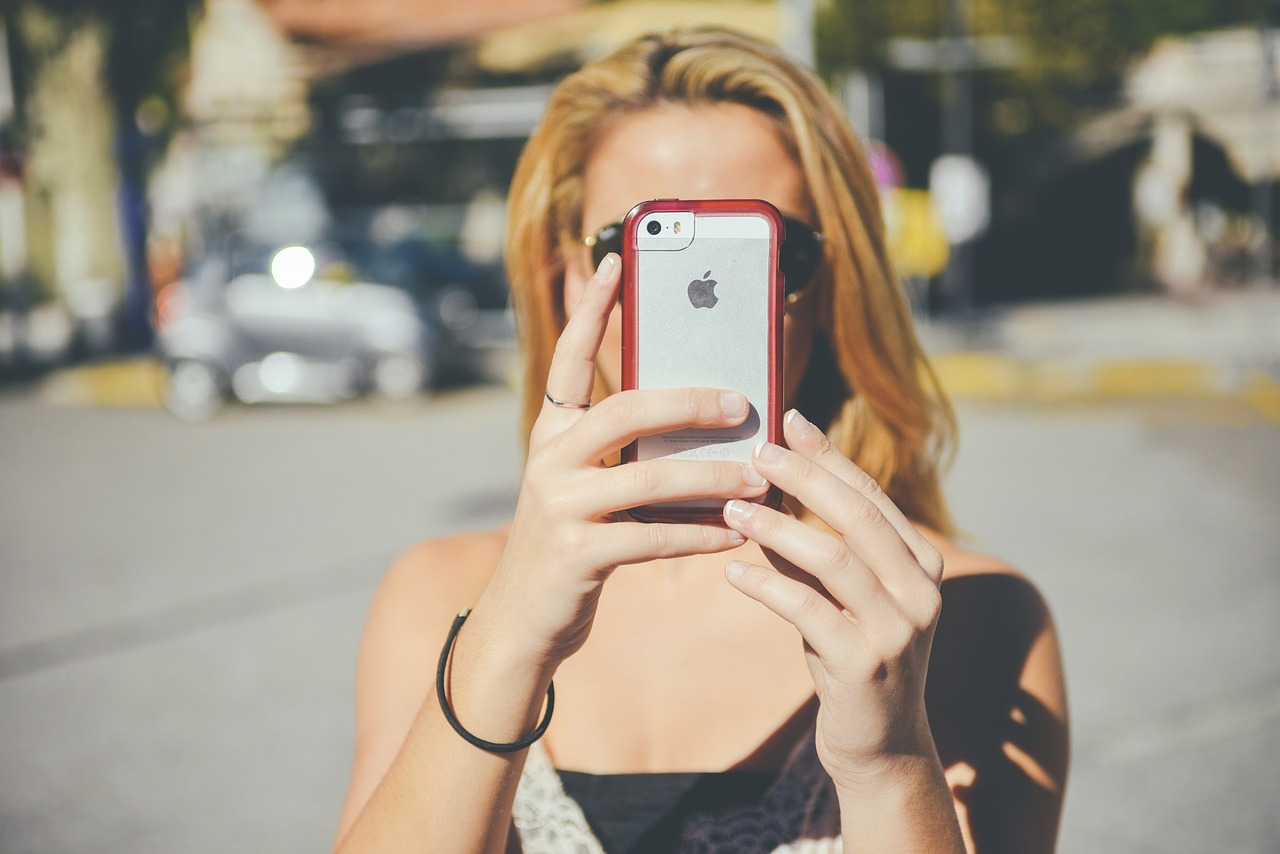
\includegraphics[width=\textwidth]{girl-1192032_1280.jpg}
\caption{Junge Frau mit einem Smartphone, Fotografie von janeb13, Pixabay}
\end{subfigure}

\caption{Telefonbenutzung früher und heute}
\end{figure}

\blindtext
\end{document}
